\documentclass[9pt]{beamer}
\usepackage{fontspec}
\usepackage[english,bulgarian]{babel}
\usepackage{xcolor}
\usepackage{amsmath}
\usepackage{mathtools} 
\usepackage{nccmath}
\usepackage{caption}
\usepackage{subfig}
\usepackage{animate}
\usepackage{xmpmulti}

\defaultfontfeatures{Ligatures=TeX}
\newfontfamily\cyrillicfont{Comfortaa-Regular}
\newfontfamily\cyrillicfonttt{Comfortaa-Regular}
\newfontfamily\fontcomic[NFSSFamily=roboto]{Roboto}
\setsansfont{Comfortaa-Regular}

\graphicspath{ {./resources/} }

\newcommand{\Q}[1]{\left[#1\right]}
\newcommand{\B}[1]{\left(#1\right)}


\usetheme{metropolis}
% \usetheme{boxes}

\begin{document}

\begin{frame}[plain, c]
    \only<1>{
        \begin{tikzpicture}[remember picture,overlay]
            \node at (current page.center) {
\includegraphics[width=\paperwidth]{1.png}};
        \end{tikzpicture}
    }
    \only<2>{
        \begin{tikzpicture}[remember picture,overlay]
        \node at (current page.center) {
\includegraphics[width=\paperwidth]{2.png}};
    \end{tikzpicture}
    }
\end{frame}

\begin{frame}{Нулева зона}
    \pause
    \begin{center}
        Първични и вторични канали за изразяване на емоция
    \end{center}
    \pause 
    \begin{itemize}
        \item[$\ $] Първичен канал - ЕЕГ
        \pause
        \item[$\ $] Вторичен канал - реч
        \begin{itemize}
            \pause 
            \item Експлицитно и имплицитно общуване
            \pause
            \item Прозодия
        \end{itemize}
        \pause
        \item Съчетаване на първичен (ЕЕГ) и вторичен (реч) канал
    \end{itemize}
\end{frame}

\section{Емоции}
\setbeamercolor{background canvas}{bg=white}
\begin{frame}
    \begin{center}
        \only<1>{
            \begin{quote}
                \textbf{Емоцията е сложна верига от събития, която започва с някакъв стимул.} В следствие настъпва фаза на ``изпитване на емоция'' и фаза на физиологични промени. Те предизвикват целенасочено държание, което цели да премахне дразнението на стимула и да върне състоянието на еквилибриум.
            \end{quote}
        }
        \only<2>{
            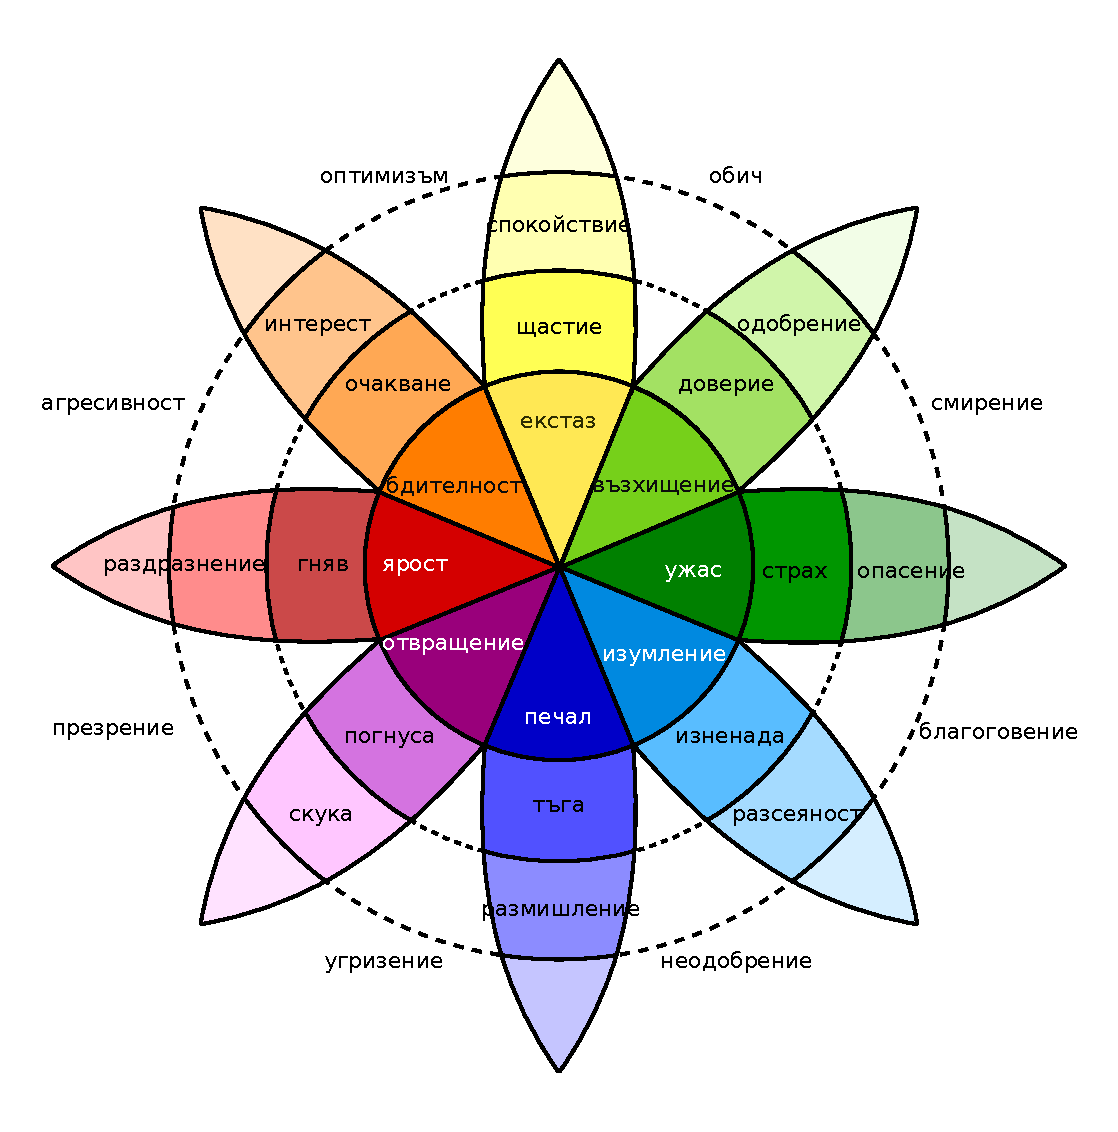
\includegraphics[width=0.8\textwidth]{plutchik}
        }%
        \only<3>{
            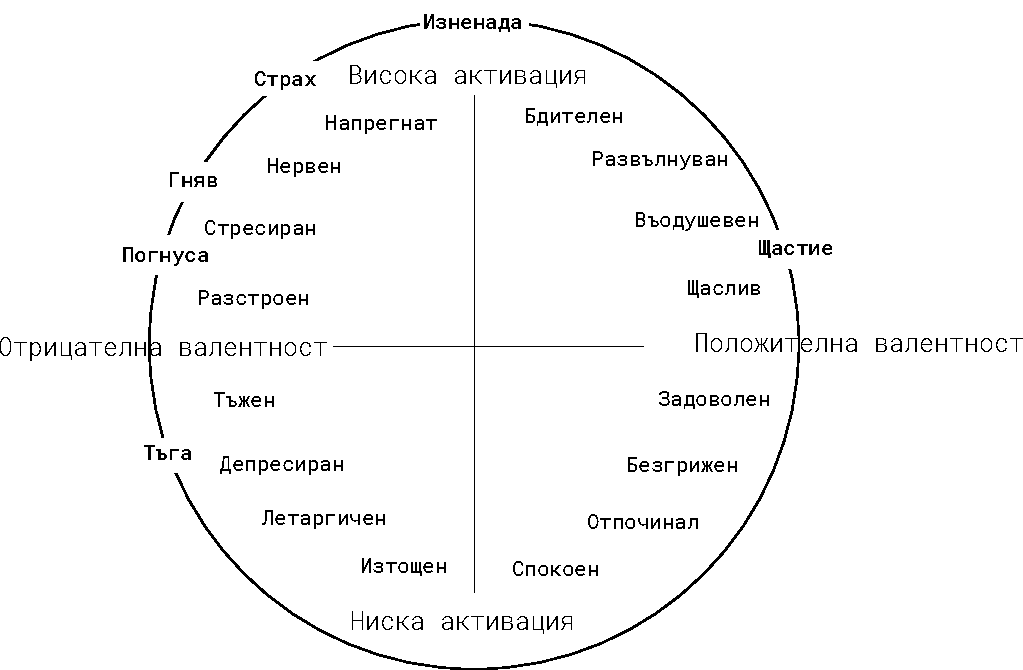
\includegraphics[width=\textwidth]{valence_arousal}
            \begin{itemize}
                \item В сигнала от реч се измерва по-лесно активацията
                \item В сигнала от ЕЕГ се измерва по-лесно валентността
            \end{itemize}
        }
    \end{center}
\end{frame}

\setbeamercolor{background canvas}{bg=white}
\begin{frame}
        \only<1>{
            \begin{columns}[T] % align columns
            \begin{column}{.38\textwidth}
            \end{column}%
            \hfill%
            \begin{column}{.60\textwidth}
                \vspace{1cm}
                \begin{center}
                    
\includegraphics[width=\textwidth]{valence_arousal_empty}%
                \end{center}
            \end{column}%
        \end{columns}
        }

        \only<2>{
            \begin{columns}[T] % align columns
            \begin{column}{.38\textwidth}
                \begin{itemize}
                    \item Гняв
                \end{itemize}
            \end{column}%
            \hfill%
            \begin{column}{.60\textwidth}
                \vspace{1cm}
                \begin{center}
                    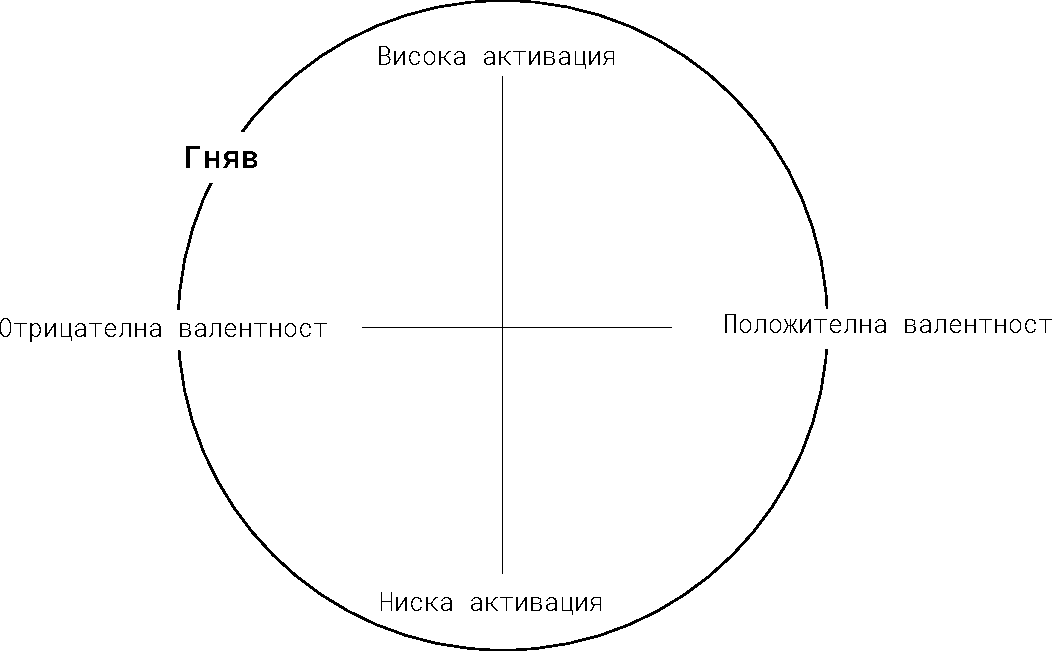
\includegraphics[width=\textwidth]{valence_arousal_a}%
                \end{center}
            \end{column}%
        \end{columns}
        }

        \only<3>{
            \begin{columns}[T] % align columns
            \begin{column}{.38\textwidth}
                \begin{itemize}
                    \item Гняв
                    \item Щастие
                \end{itemize}
            \end{column}%
            \hfill%
            \begin{column}{.60\textwidth}
                \vspace{1cm}
                \begin{center}
                    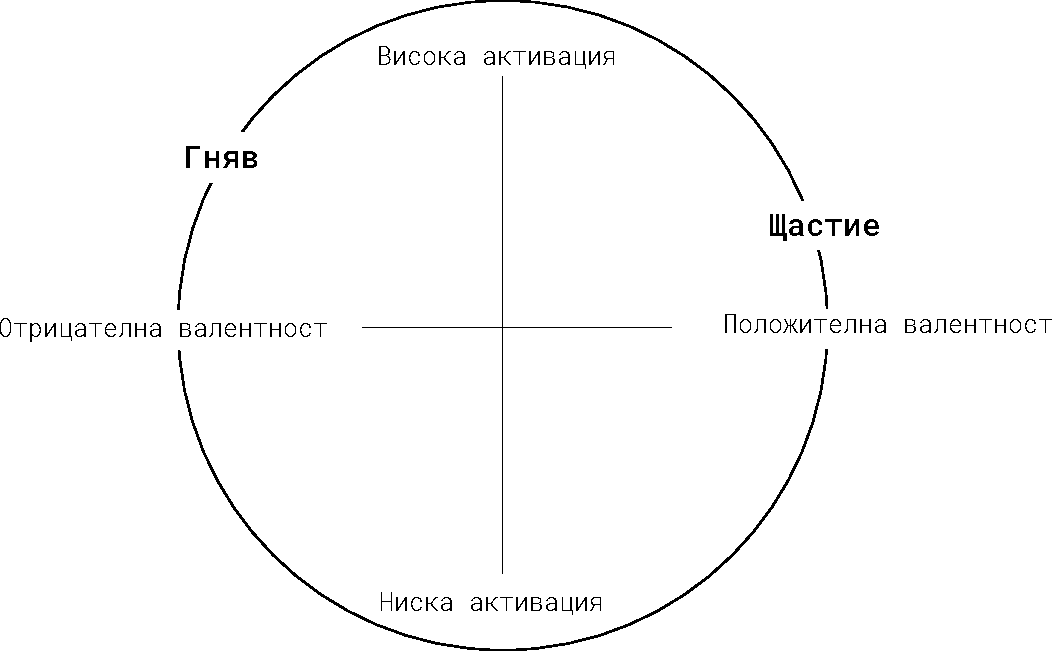
\includegraphics[width=\textwidth]{valence_arousal_ah}%
                \end{center}
            \end{column}%
        \end{columns}
        }

        \only<4>{
            \begin{columns}[T] % align columns
            \begin{column}{.38\textwidth}
                \begin{itemize}
                    \item Гняв
                    \item Щастие
                    \item Неутрална емоция
                \end{itemize}
            \end{column}%
            \hfill%
            \begin{column}{.60\textwidth}
                \vspace{1cm}
                \begin{center}
                    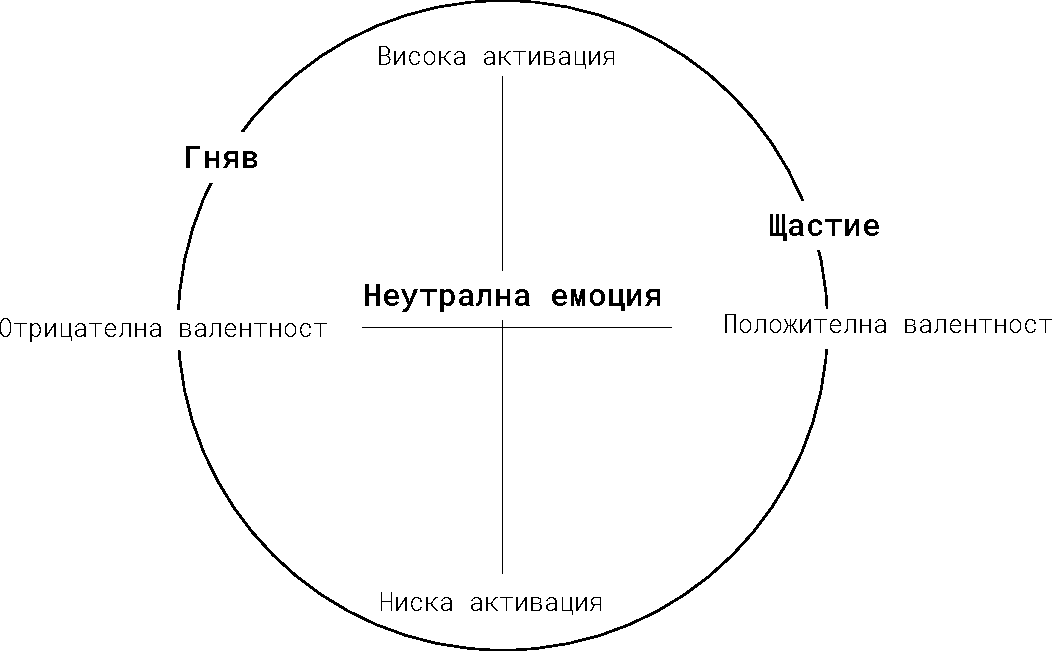
\includegraphics[width=\textwidth]{valence_arousal_ahn}%
                \end{center}
            \end{column}%
        \end{columns}
        }

        \only<5>{
            \begin{columns}[T] % align columns
            \begin{column}{.38\textwidth}
                \begin{itemize}
                    \item Гняв
                    \item Щастие
                    \item Неутрална емоция
                    \item Тъга
                \end{itemize}
            \end{column}%
            \hfill%
            \begin{column}{.60\textwidth}
                \vspace{1cm}
                \begin{center}
                    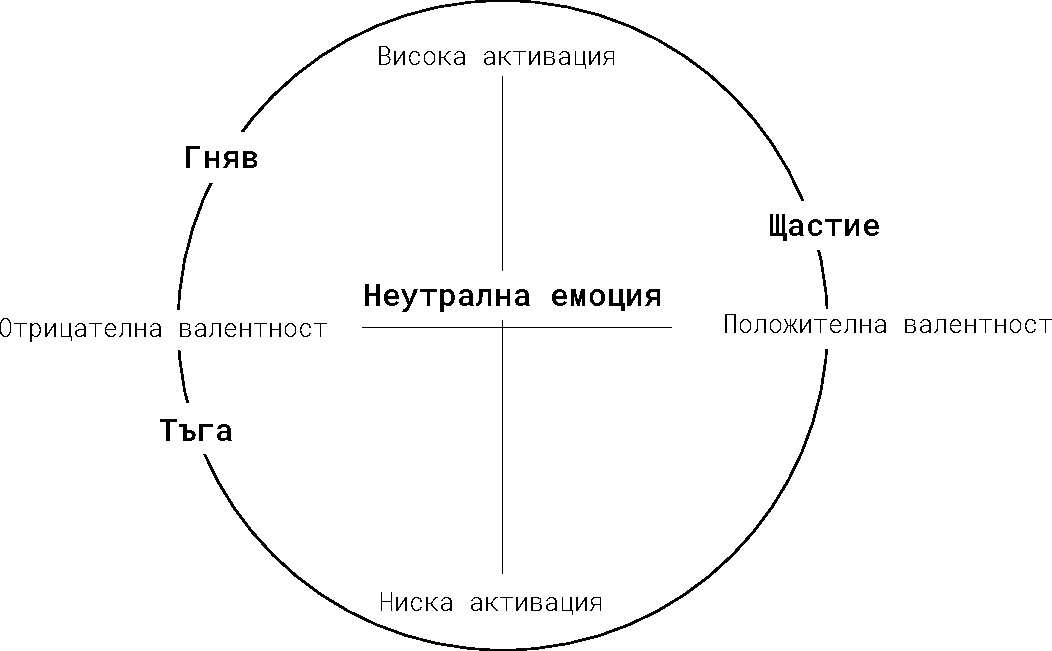
\includegraphics[width=\textwidth]{valence_arousal_ahns}%
                \end{center}
            \end{column}%
        \end{columns}
        }
\end{frame}

\section{Реч}
\begin{frame}[b]
    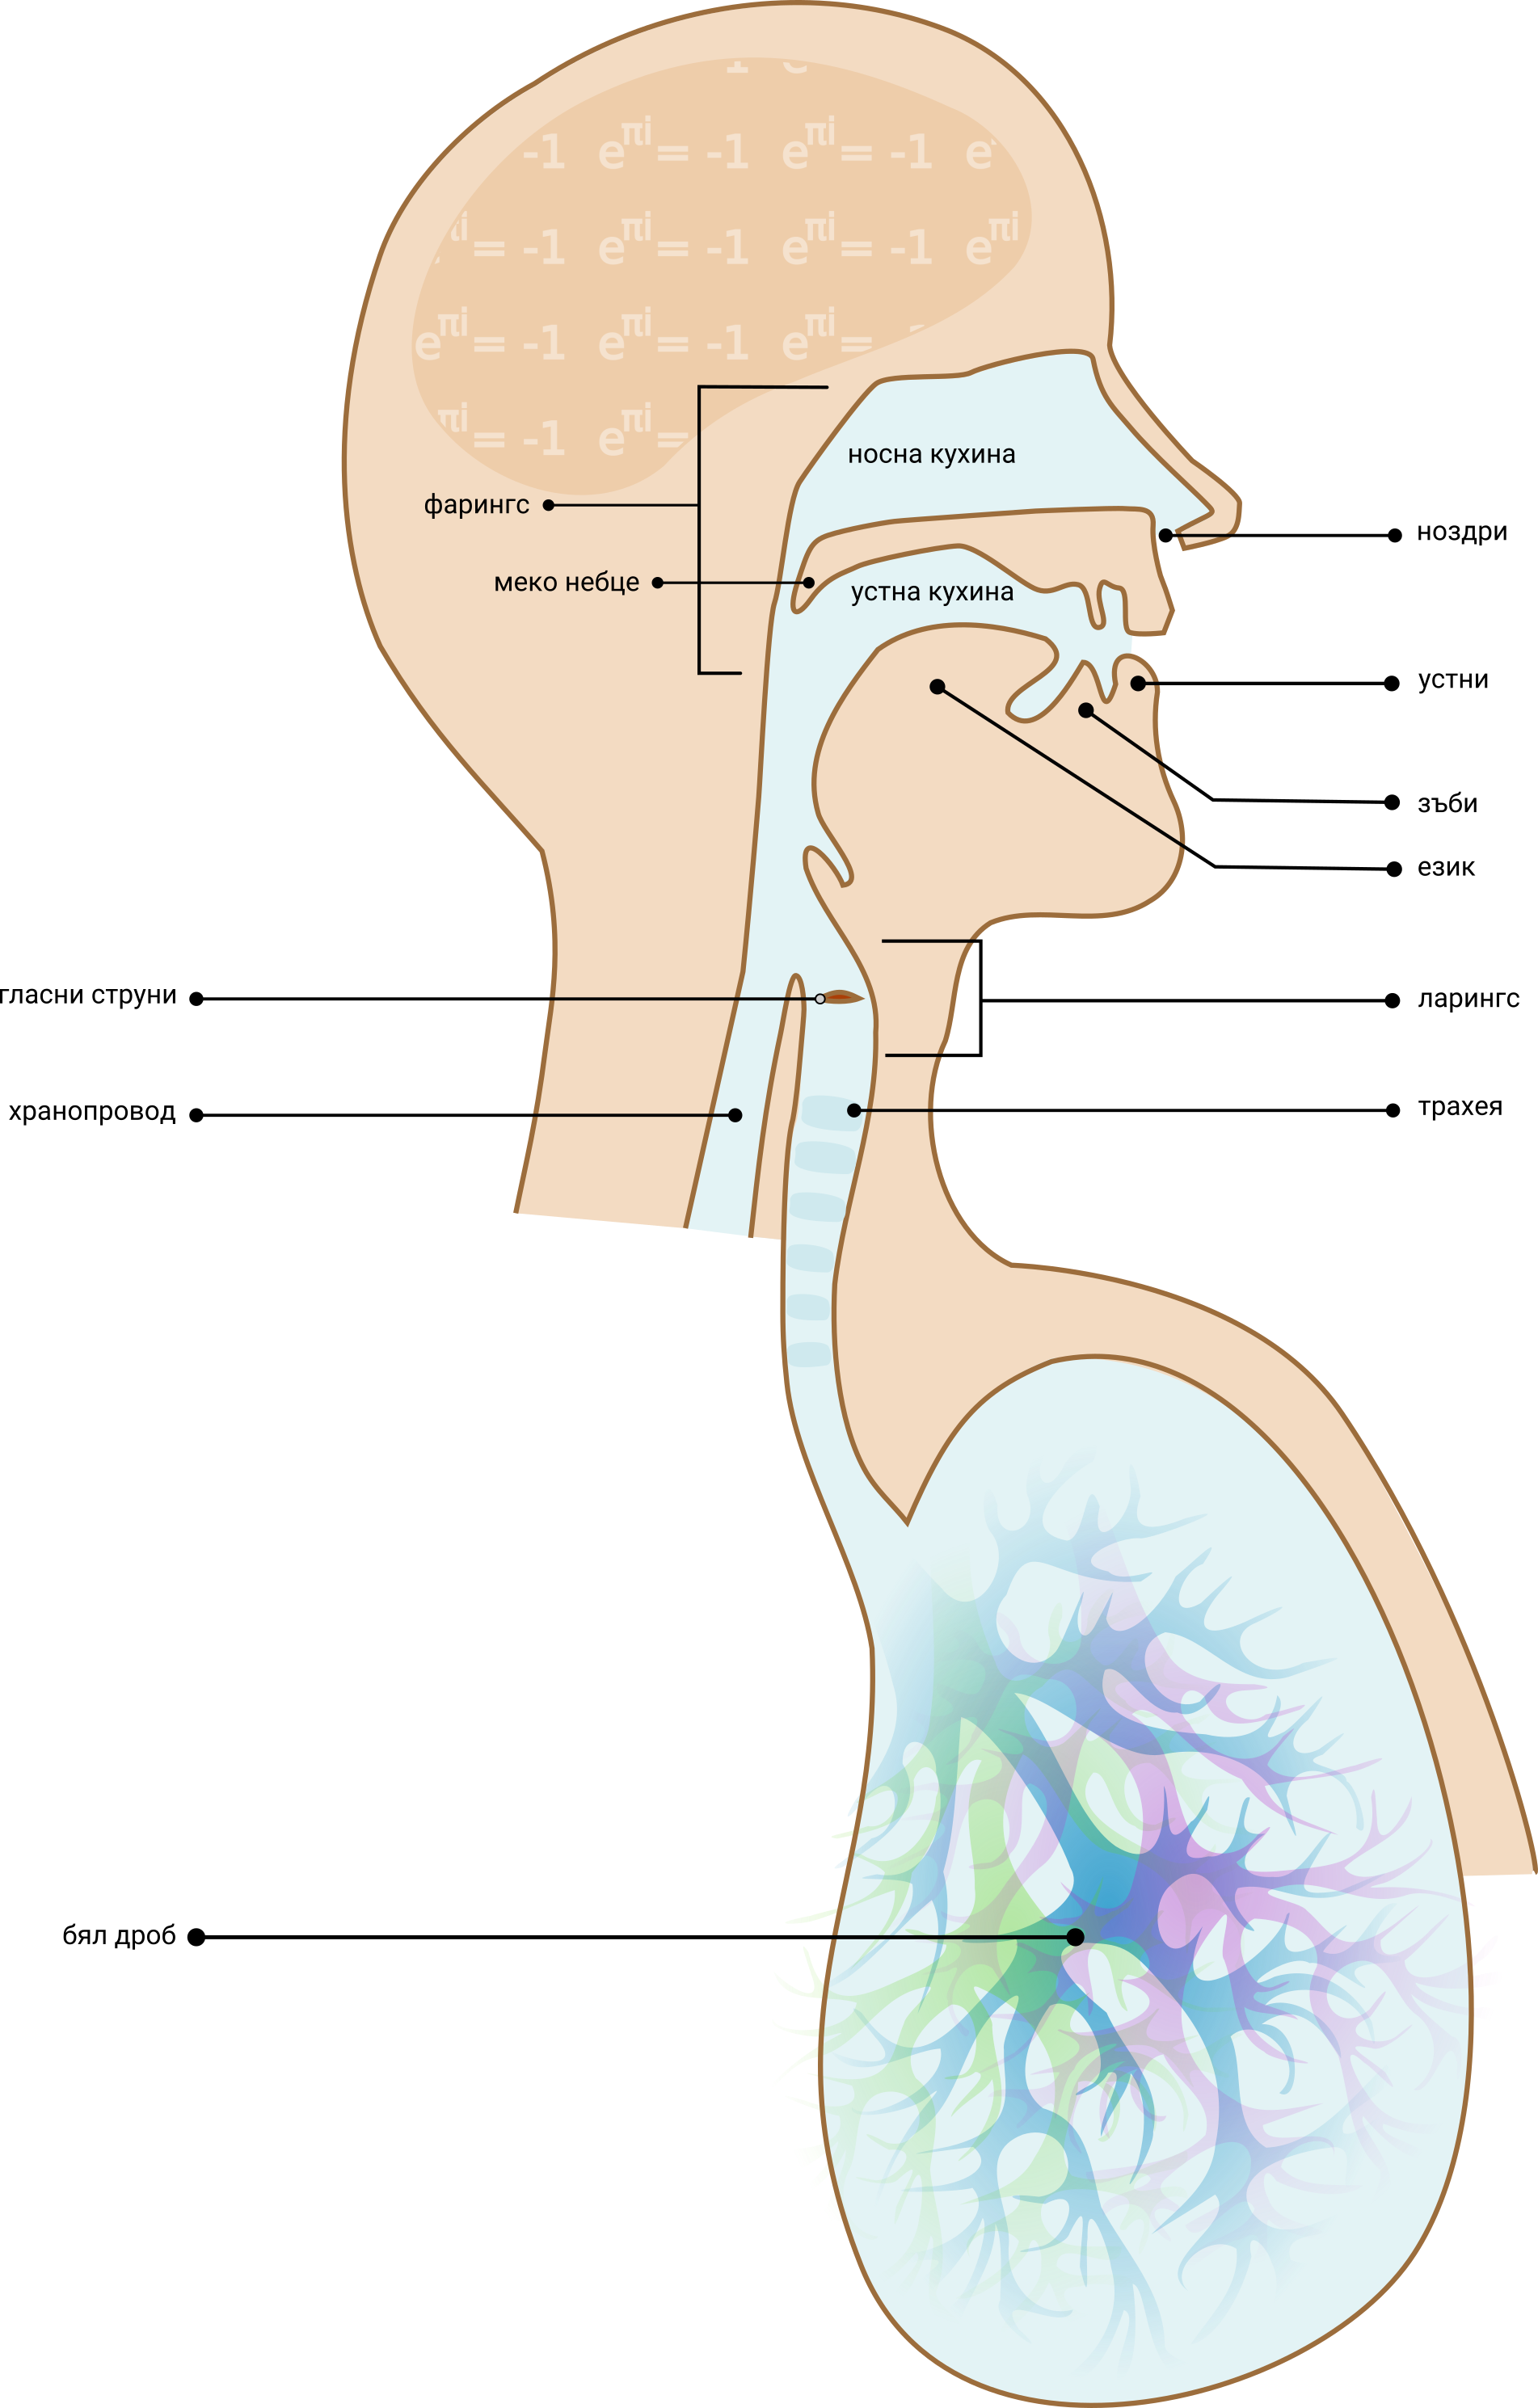
\includegraphics[width=0.48\paperwidth]{physics}%
    \hfill
    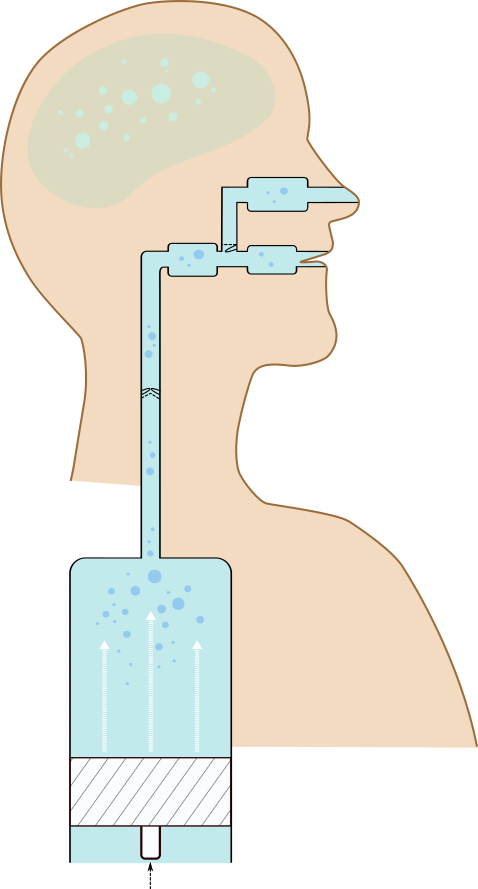
\includegraphics[width=0.28\paperwidth]{tubes}
\end{frame}

\begin{frame}
    \begin{itemize}
        \only<1>{
                 \item  Глотисът \alert{g} трепти, вокалният тракт \alert{v} филтрира сигнала, и вълната излиза и допълнително се променя от устните \alert{r}
                 }
        \only<2->{
                    \item  Глотисът $\textbf{g}$ трепти, вокалният тракт $\textbf{v}$ филтрира сигнала, и вълната излиза и допълнително се променя от устните $\textbf{r}$
                 }
        \only<2>{
                 \item[$\ $] Ако  $g(t) \xleftrightarrow{\mathcal{F}\mathcal{S}} \mathcal{G}(z), v(t) \xleftrightarrow{\mathcal{F}\mathcal{S}} \mathcal{V}(z), r(t) \xleftrightarrow{\mathcal{F}\mathcal{S}} \mathcal{R}(z)$, а сигналът, който получаваме накрая,\\
                 $y(t)=g(t)\ast v(t) \ast r(t), y(t) \xleftrightarrow{\mathcal{F}\mathcal{S}} \mathcal{Y}(z)$, е изпълнено, че
                 }
        \only<3->{
                    \item[$\ $] Ако  $g(t) \xleftrightarrow{\mathcal{F}\mathcal{S}} \mathcal{G}(z), v(t) \xleftrightarrow{\mathcal{F}\mathcal{S}} \mathcal{V}(z), r(t) \xleftrightarrow{\mathcal{F}\mathcal{S}} \mathcal{R}(z)$, а сигналът, който получаваме накрая,\\
                    $y(t)=g(t)\ast v(t) \ast r(t), y(t) \xleftrightarrow{\mathcal{F}\mathcal{S}} \mathcal{Y}(z)$, е изпълнено, че
                 }
        \only<3>{
                 \item $\mathcal{Y}(z) = \mathcal{G}(z) \mathcal{V}(z) \mathcal{R}(z)$
                }
        \only<4>{
            \item $\mathcal{Y}(z) = \mathcal{G}(z) \alert{\mathcal{V}(z) \mathcal{R}(z)}$
        }  
        \only<5>{
                \item $\mathcal{Y}(z) = \mathcal{G}(z) \mathcal{H}(z)$
        }
    \end{itemize}
\end{frame}

\begin{frame}[t]
    \begin{itemize}
        \only<1> {
            \item[$\ $] $\alert{\mathcal{Y}(z) = \mathcal{G}(z) \mathcal{H}(z)}$
        }
        \only<2-> {
            \item[$\ $] $\mathcal{Y}(z) = \mathcal{G}(z) \mathcal{H}(z)$
        }
        \only<2> {
            \item Модел на тръбите
        }
        \only<3-> {
            \item Модел на тръбите
        }
        \only<3>{\item Уравнения на Навие-Стокс:

            \begin{flalign*}
                -\frac{\partial\rho}{\partial x} & = \frac{\rho}{A} \frac{\partial u}{\partial t} && \\
                -\frac{\partial u}{\partial x} & = \frac{A}{\rho c^2} \frac{\partial \rho}{\partial t} && 
            \end{flalign*}
        }
        \only<4->{\item Уравнения на Навие-Стокс:
        
            \begin{flalign*}
                -\frac{\partial\rho}{\partial x} & = \frac{\rho}{A} \frac{\partial u}{\partial t} && \\
                -\frac{\partial u}{\partial x} & = \frac{A}{\rho c^2} \frac{\partial \rho}{\partial t} && 
            \end{flalign*}
        }
        \only<4>{\item $\mathcal{Y}(z) = \mathcal{G}(z) \cfrac{\sum\limits_{m=0}^{M} b_m z^{-m} }{\sum\limits_{k=0}^{K} a_k z^{-k}}\hfill z = e^{i\omega}$}

    \end{itemize}
\end{frame}

\begin{frame}[t]
    \begin{itemize}
        \only<1> {
            \item[$\ $] $\mathcal{Y}(z) = \mathcal{G}(z) \mathcal{H}(z)$
        }
        \only<2-> {
            \item[$\ $] $\mathcal{Y}(z) = \mathcal{G}(z) \mathcal{H}(z)$
        }
        \only<2> { \item $log(|\mathcal{Y}(z)|) = log(|\mathcal{G}(z)|) + log(|\mathcal{H}(z)|)$
        }
        \only<3-> {
            \item $log(|\mathcal{Y}(z)|) = log(|\mathcal{G}(z)|) + log(|\mathcal{H}(z)|)$
        }
        \only<3> {
            \begin{columns}
                \begin{column}{0.48\textwidth}
                     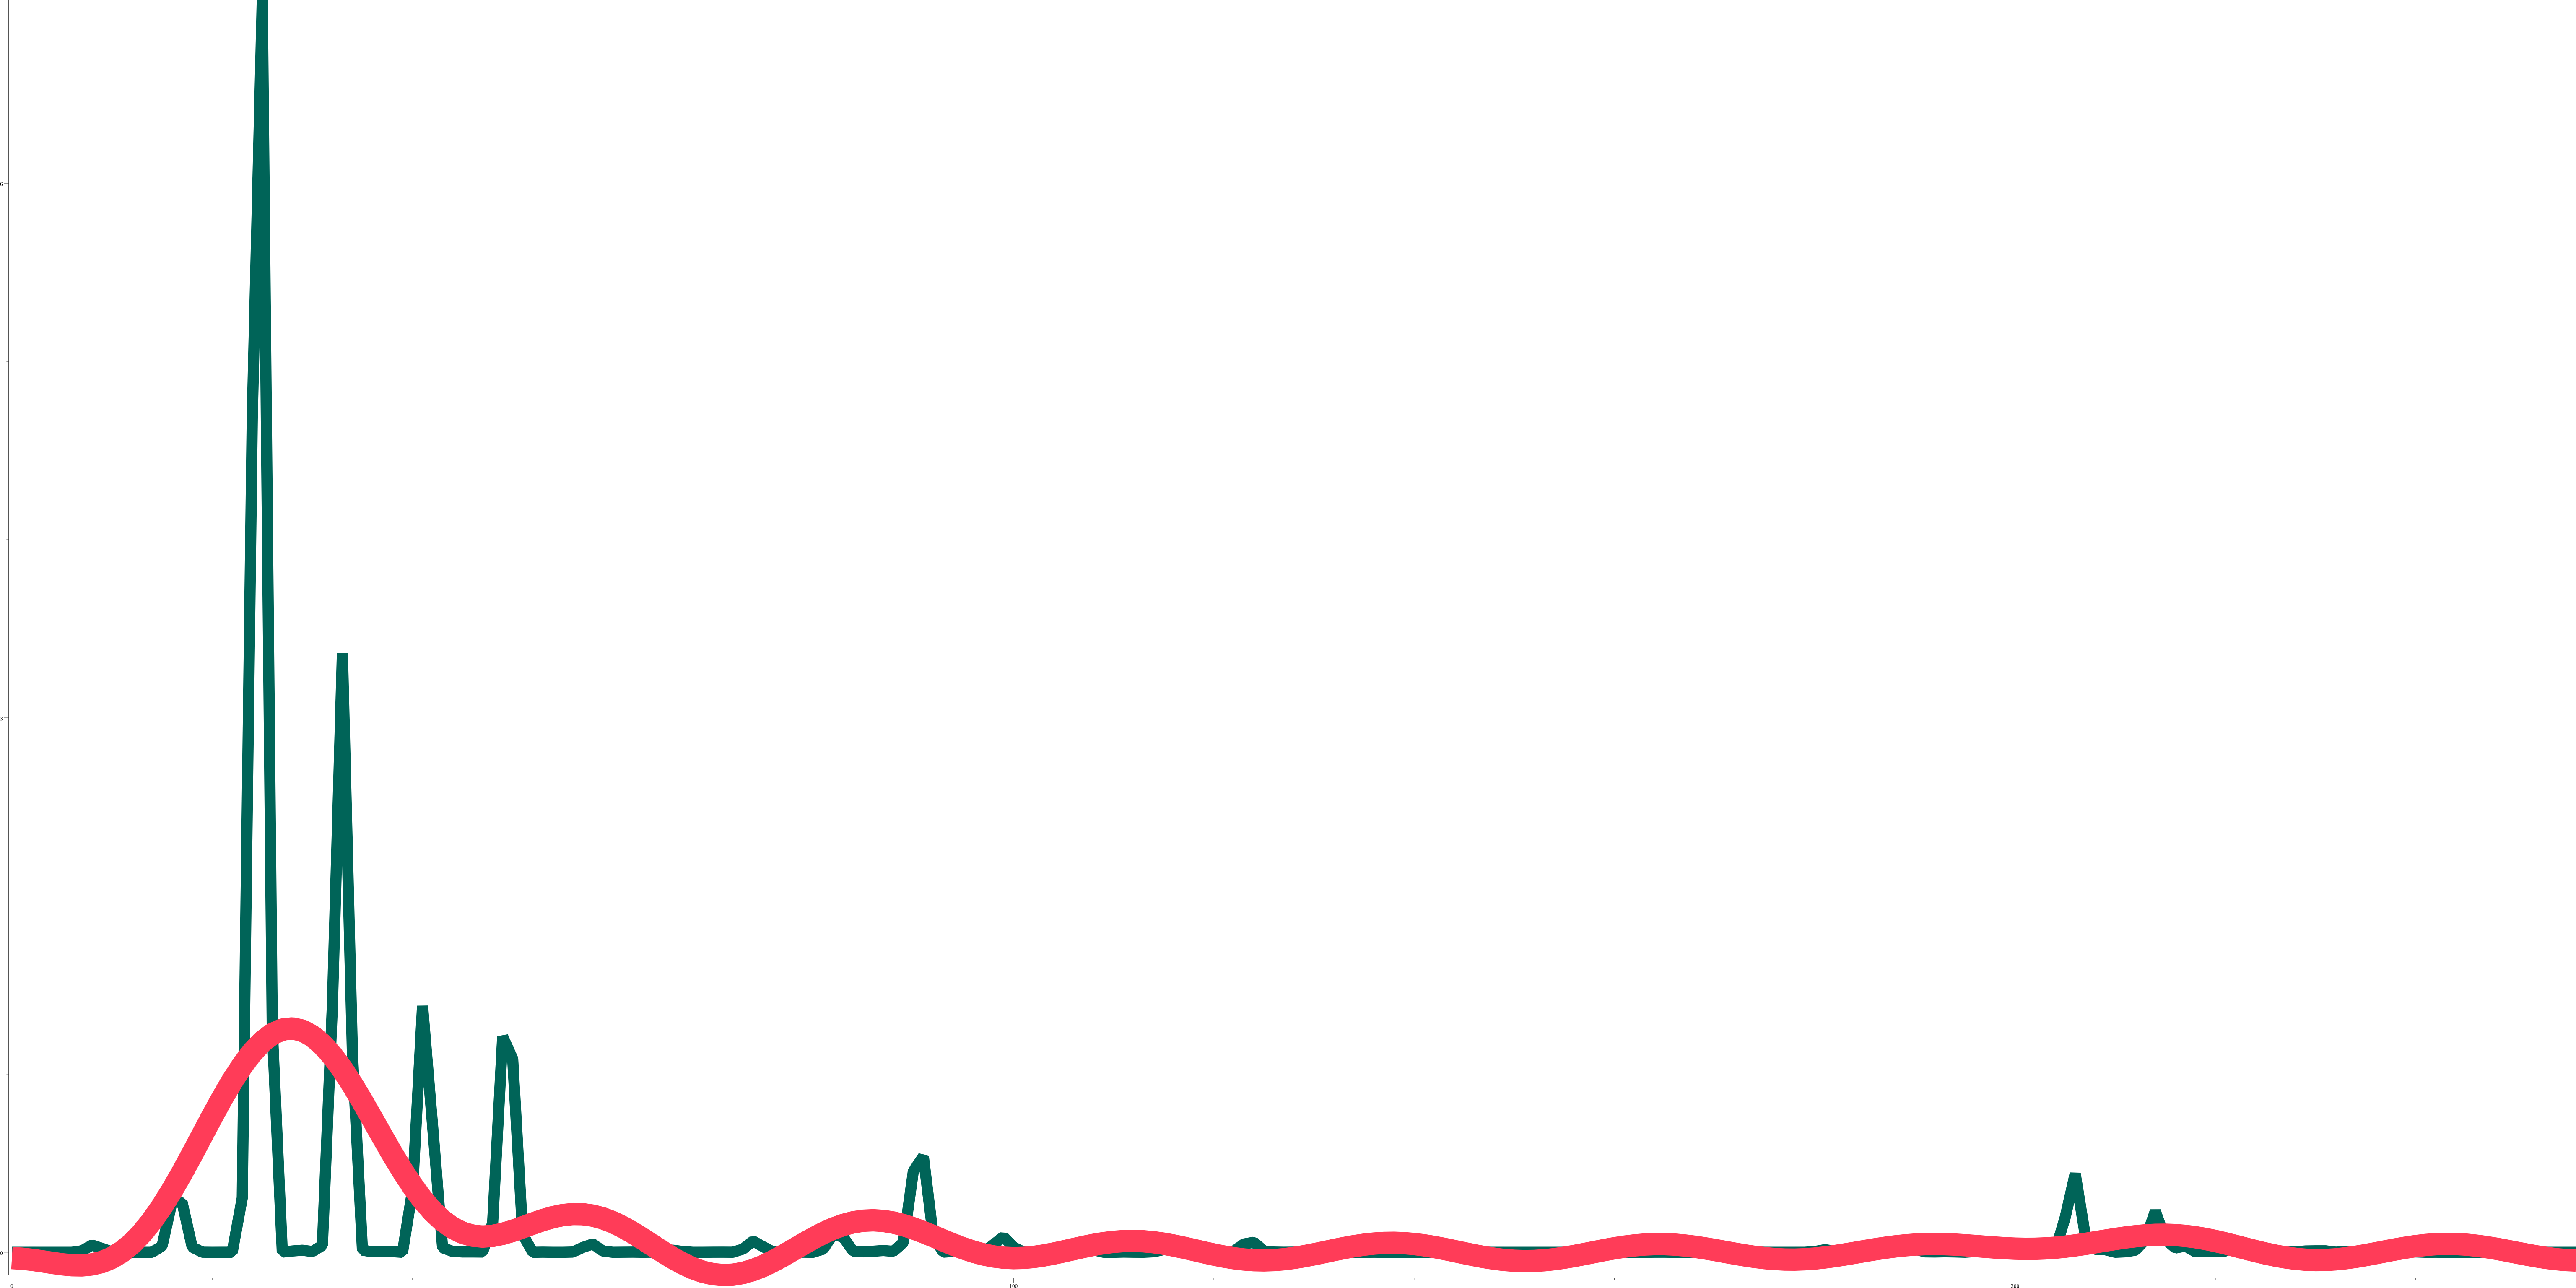
\includegraphics[width=\textwidth]{aaaa.png}
                \end{column}
                \pause
                \hfill
                \begin{column}{0.48\textwidth}
                    %  \includegraphics[width=\textwidth]{aaaa_log.png}
                \end{column}
            \end{columns}
        }
        \only<4> {
                \begin{columns}
                    \begin{column}{0.48\textwidth}
                         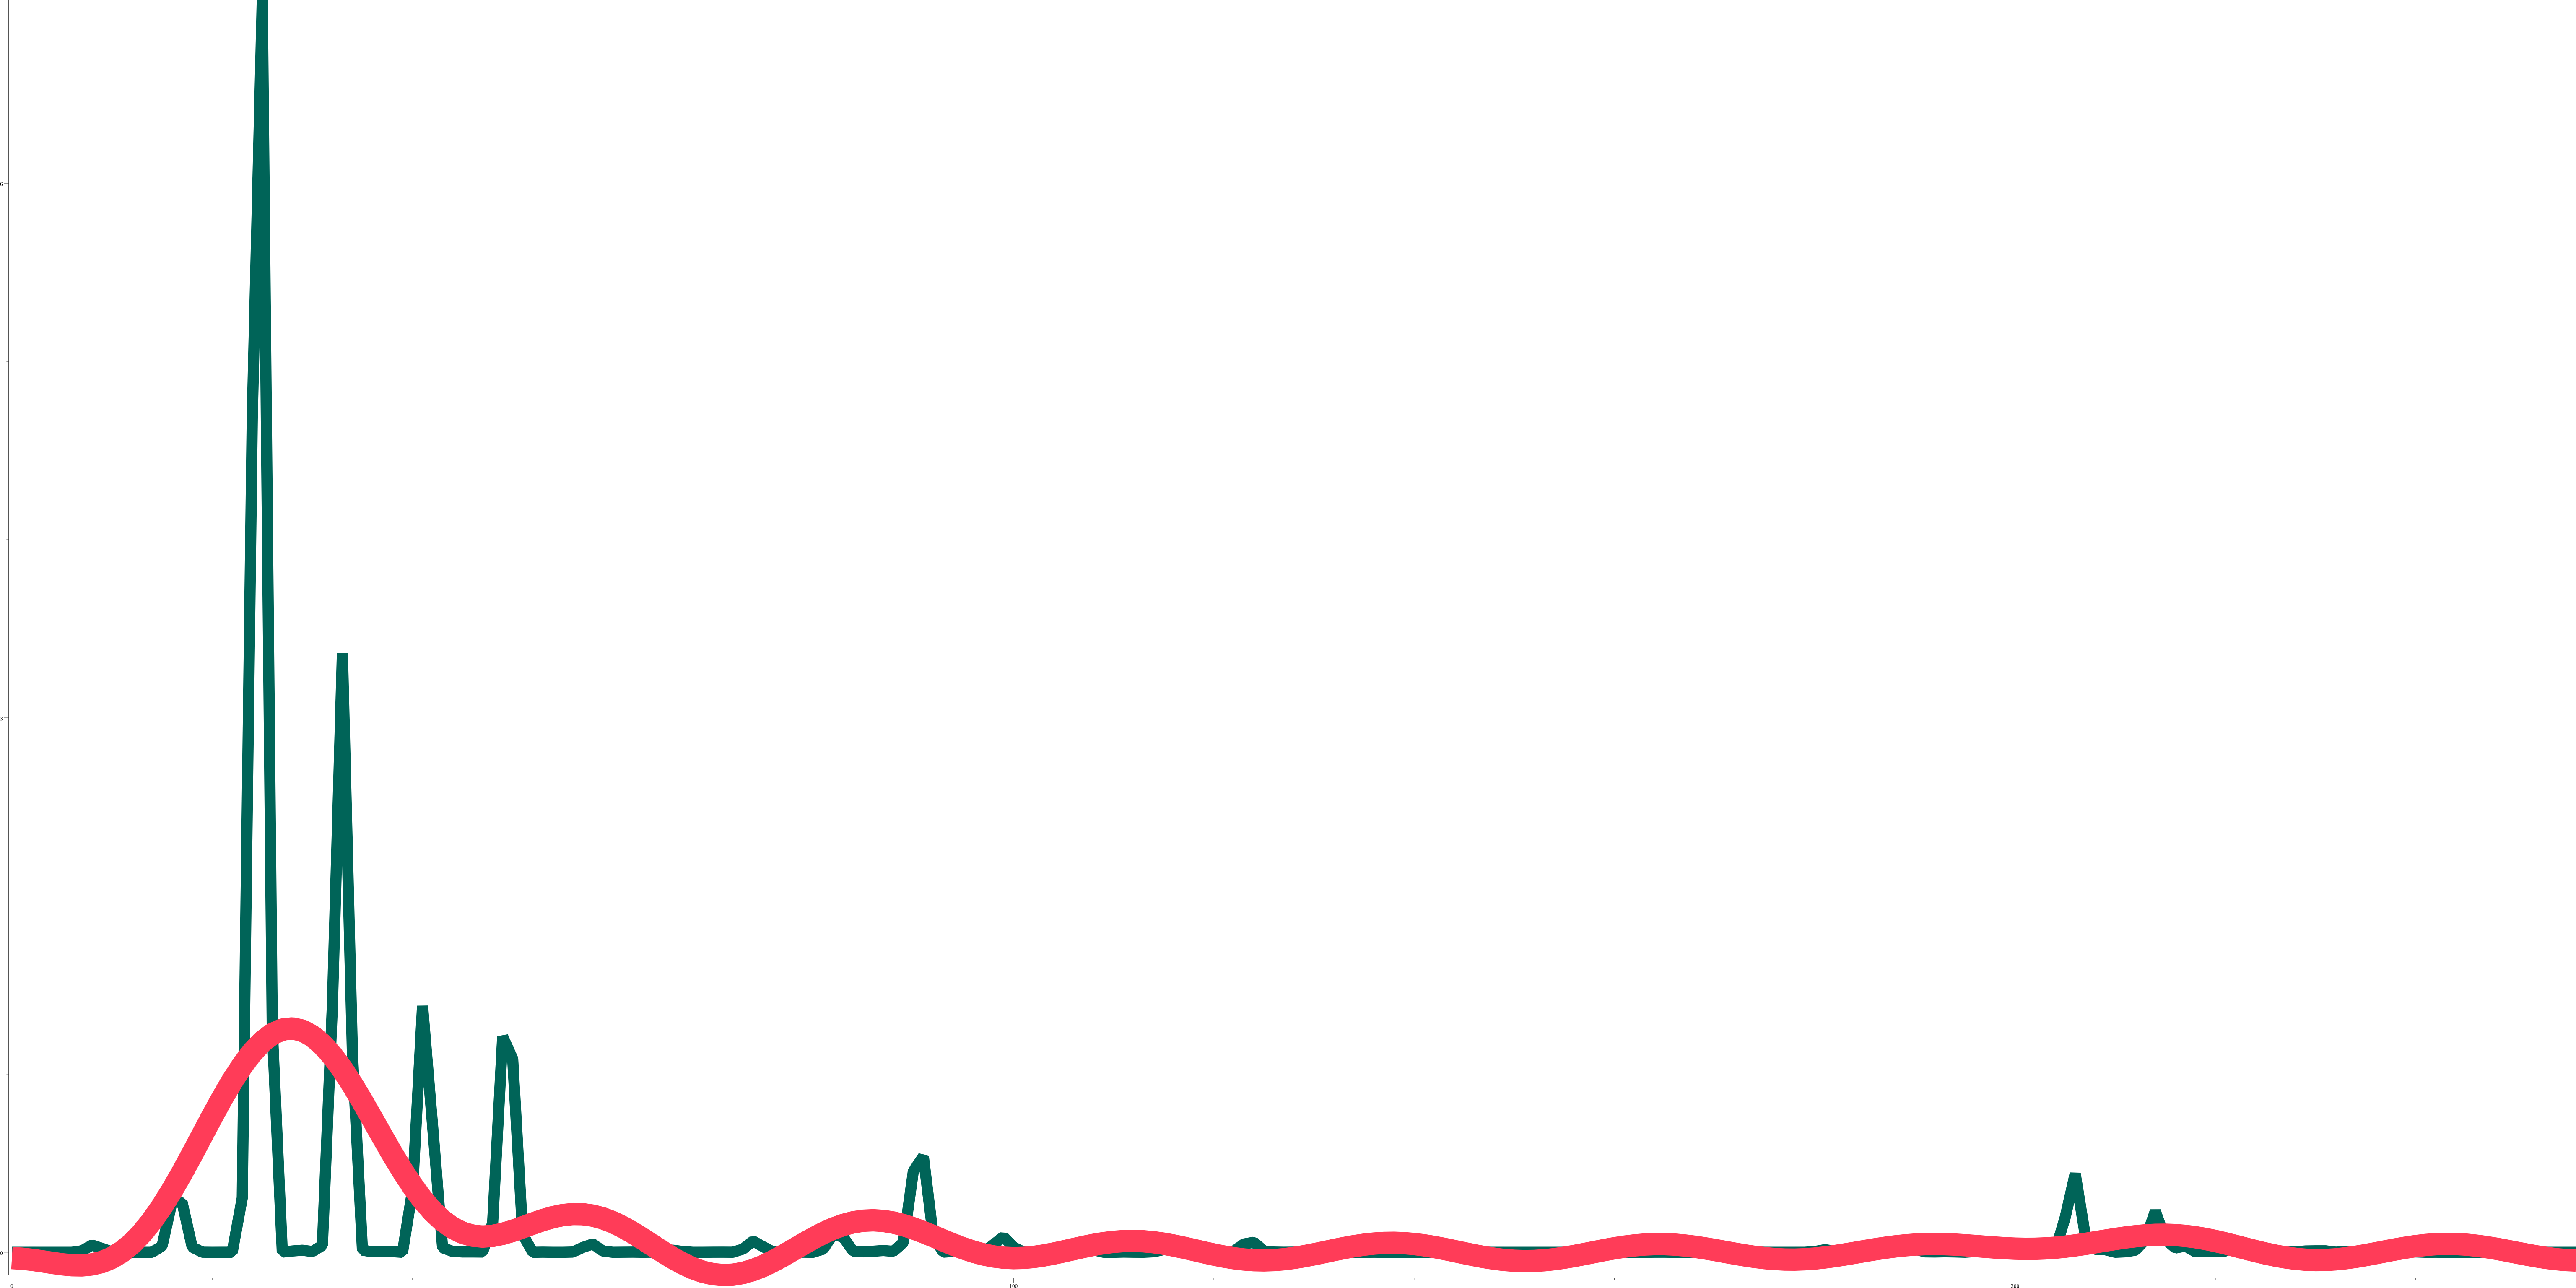
\includegraphics[width=\textwidth]{aaaa.png}
                    \end{column}
                    \pause
                    \hfill
                    \begin{column}{0.48\textwidth}
                         \includegraphics[width=\textwidth]{aaaa_log.png}
                    \end{column}
                \end{columns}
        }
        \only<5-> {
                \begin{columns}
                    \begin{column}{0.48\textwidth}
                         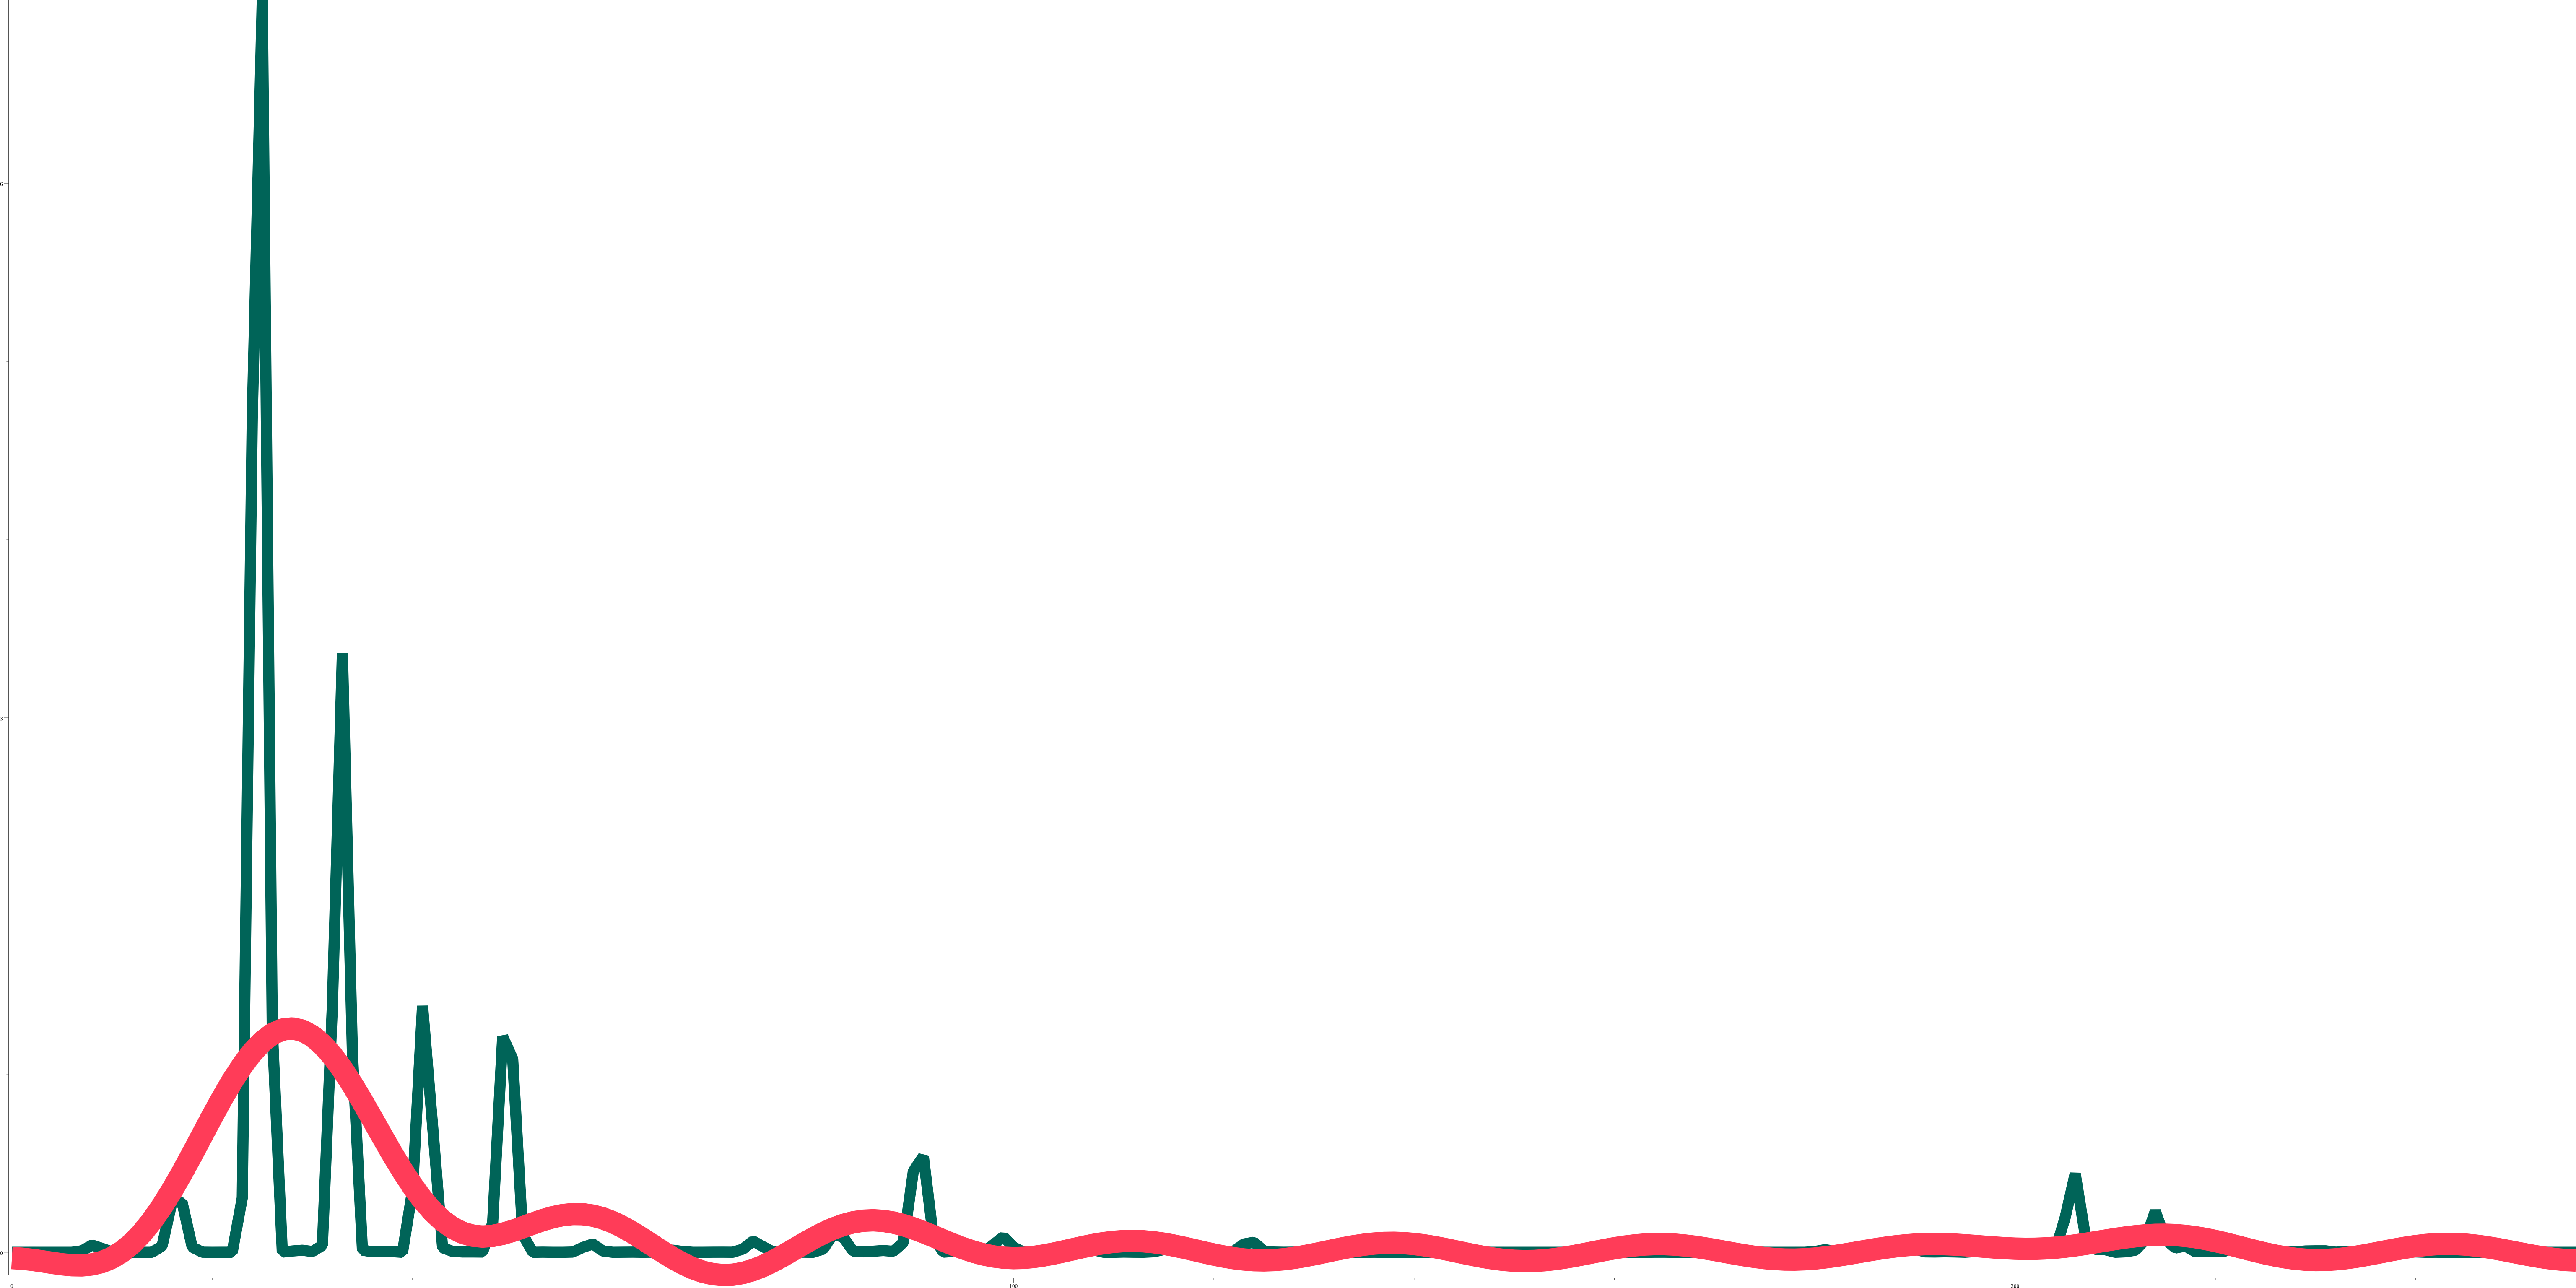
\includegraphics[width=\textwidth]{aaaa.png}
                    \end{column}
                    \pause
                    \hfill
                    \begin{column}{0.48\textwidth}
                         \includegraphics[width=\textwidth]{aaaa_log.png}
                    \end{column}
                \end{columns}
        }
        \only<5-12> {
            \item<5-12> Обратно Фурие преобразувание - кепстър
            \item<6-12> $c_y[n] = c_g[n] + c_h[n]$
            \item<7-12> $c_g[n]$ ще са във високите честоти
            \item<8-12> $c_h[n]$ ще са в ниските
            \item<9-12> Използване на логаритимична (Мел) скала
            \item<10-12> Натрупване в критични области
            \item<11-12> Първите 13 MFCC коефициента и техните крайни разлики от първи и втори ред
            \item<12-12> 39-мерни вектори
            }
    \end{itemize}
\end{frame}

\section{Класификация}
\begin{frame}[t]
    \begin{itemize}
        \item Гаусови смески
        \pause - всяко непрекъснато разпределение върху $\mathbb{R}^{n}$ може да се приближи произволно точно с линейна комбинация на достатъчно на брой гаусиани
        \pause
        \item За всяка емоция $e$ имаме по една смеска $(\hat{\pi}^e, \hat{\mu}^e, \hat{\Sigma}^e)$
        \pause
        \item При подаден характеристичен вектор $x$, вероятностната плътност на смеска е:
        \pause

        $p(x) = \sum\limits_{k=1}^{K} \pi_k^e \mathcal{N}(x; \mu_k^e, \Sigma_k^e)$
        \pause
        \item Правдоподобието на всички вектори X с етикет $e$ спрямо $(\hat{\pi}^e, \hat{\mu}^e, \hat{\Sigma}^e)$:
        \pause    
    
        $p(X|(\hat{\pi}^e, \hat{\mu}^e, \hat{\Sigma}^e)) = \prod\limits_{i=1}^{n} \sum\limits_{k=1}^{K} \pi_k^e \mathcal{N}(x_i; \mu_k^e, \Sigma_k^e)$.
        \pause
        \item За всяка емоция намираме Гаусовата смеска, която максимизира логаритъм от правдоподобието на съответните вектори
        \pause - ЕМ метод
    \end{itemize}
\end{frame}

\section{Бази данни и резултати (реч)}
    \begin{frame}[t]
        \begin{itemize}
            \item Emo-DB
            \pause - 800 записа от 10 актьори
        \end{itemize}
        \pause
        \begin{center}
            \resizebox{0.6\textwidth}{!}{\begin{tabular}{|l|r|r|} 
                \hline
                Емоция & Брой файлове & Обща дължина\\ 
                \hline
                Гняв & 127 & 5 мин. 35 сек.\\ 
                Щастие &  71 & 3 мин. 00 сек.\\ 
                Неутрално състояние &  79 & 3 мин. 06 сек.\\ 
                Тъга &  61 & 4 мин. 05 сек.\\ 
                \hline
            \end{tabular}}
        \end{center}
        \pause
        \begin{table}[h]
            \begin{center}
                \resizebox{\textwidth}{!}{\begin{tabular}{ |l|c|c|l| } 
                 \hline
                 Източник & Тип класификатор &  Тип характеристични вектори & Резултат \\ 
                 \hline
                 Текущ & GMM & MFCC & 82.20\% \\ 
                 2011 & SVM & LPCMFCC & 82.50\% \\ 
                 2006 &  Naïve Bayes classifier & MFCC & 82.76\% \\ 
                 2017 &  Random forest & MFCC & 79.02\% \\ 
                 \hline
                \end{tabular}}
                \caption*{Резултати върху emo-DB}
                \end{center}
        \end{table}
    \end{frame}

    \begin{frame}[t]
        \pause
        \begin{itemize}
            \item Тази сутрин-DB
        \end{itemize}
        \pause
        \begin{center}
            \resizebox{0.8\textwidth}{!}{\begin{tabular}{|l|r|r|} 
                \hline
                Емоция & Брой файлове & Обща дължина\\ 
                \hline
                Гняв & 51 & 4 мин. 15 сек.\\ 
                Щастие &  33 & 2 мин. 45 сек.\\ 
                Неутрално състояние &  18 & 1 мин. 30 сек.\\ 
                Тъга &  22 & 1 мин. 59 сек.\\ 
                \hline
            \end{tabular}}
        \end{center}
    \pause
    \begin{table}[h]
        \begin{center}
            \resizebox{0.8\textwidth}{!}{\begin{tabular}{|l|r r r r|} 
                \hline
                & Гняв & Щастие & Неутрално & Тъга\\ 
                \hline
                Гняв &  \textbf{72.00\%} & 4.00\% & 12.00\% & 12.00\%\\ 
                Щастие & 10.00\% & \textbf{73.33\%} & 0.00\% & 16.67\% \\ 
                Неутрално & 6.67\% & 6.67\% & \textbf{67.67\%} & 20.00\% \\ 
                Тъга & 0.00\% & 0.00\% & 0.00\% & \textbf{100.00\%}\\ 
                \hline
                \hline
                Общо & & & & \textbf{78.00\%}\\
                \hline
            \end{tabular}}
            \caption*{Матрица на грешките за база данни от ``Тази сутрин'' на ниво файл}
        \end{center}
        \end{table}
    \end{frame}

    \section{ЕЕГ}
    \begin{frame}[t]
        \center{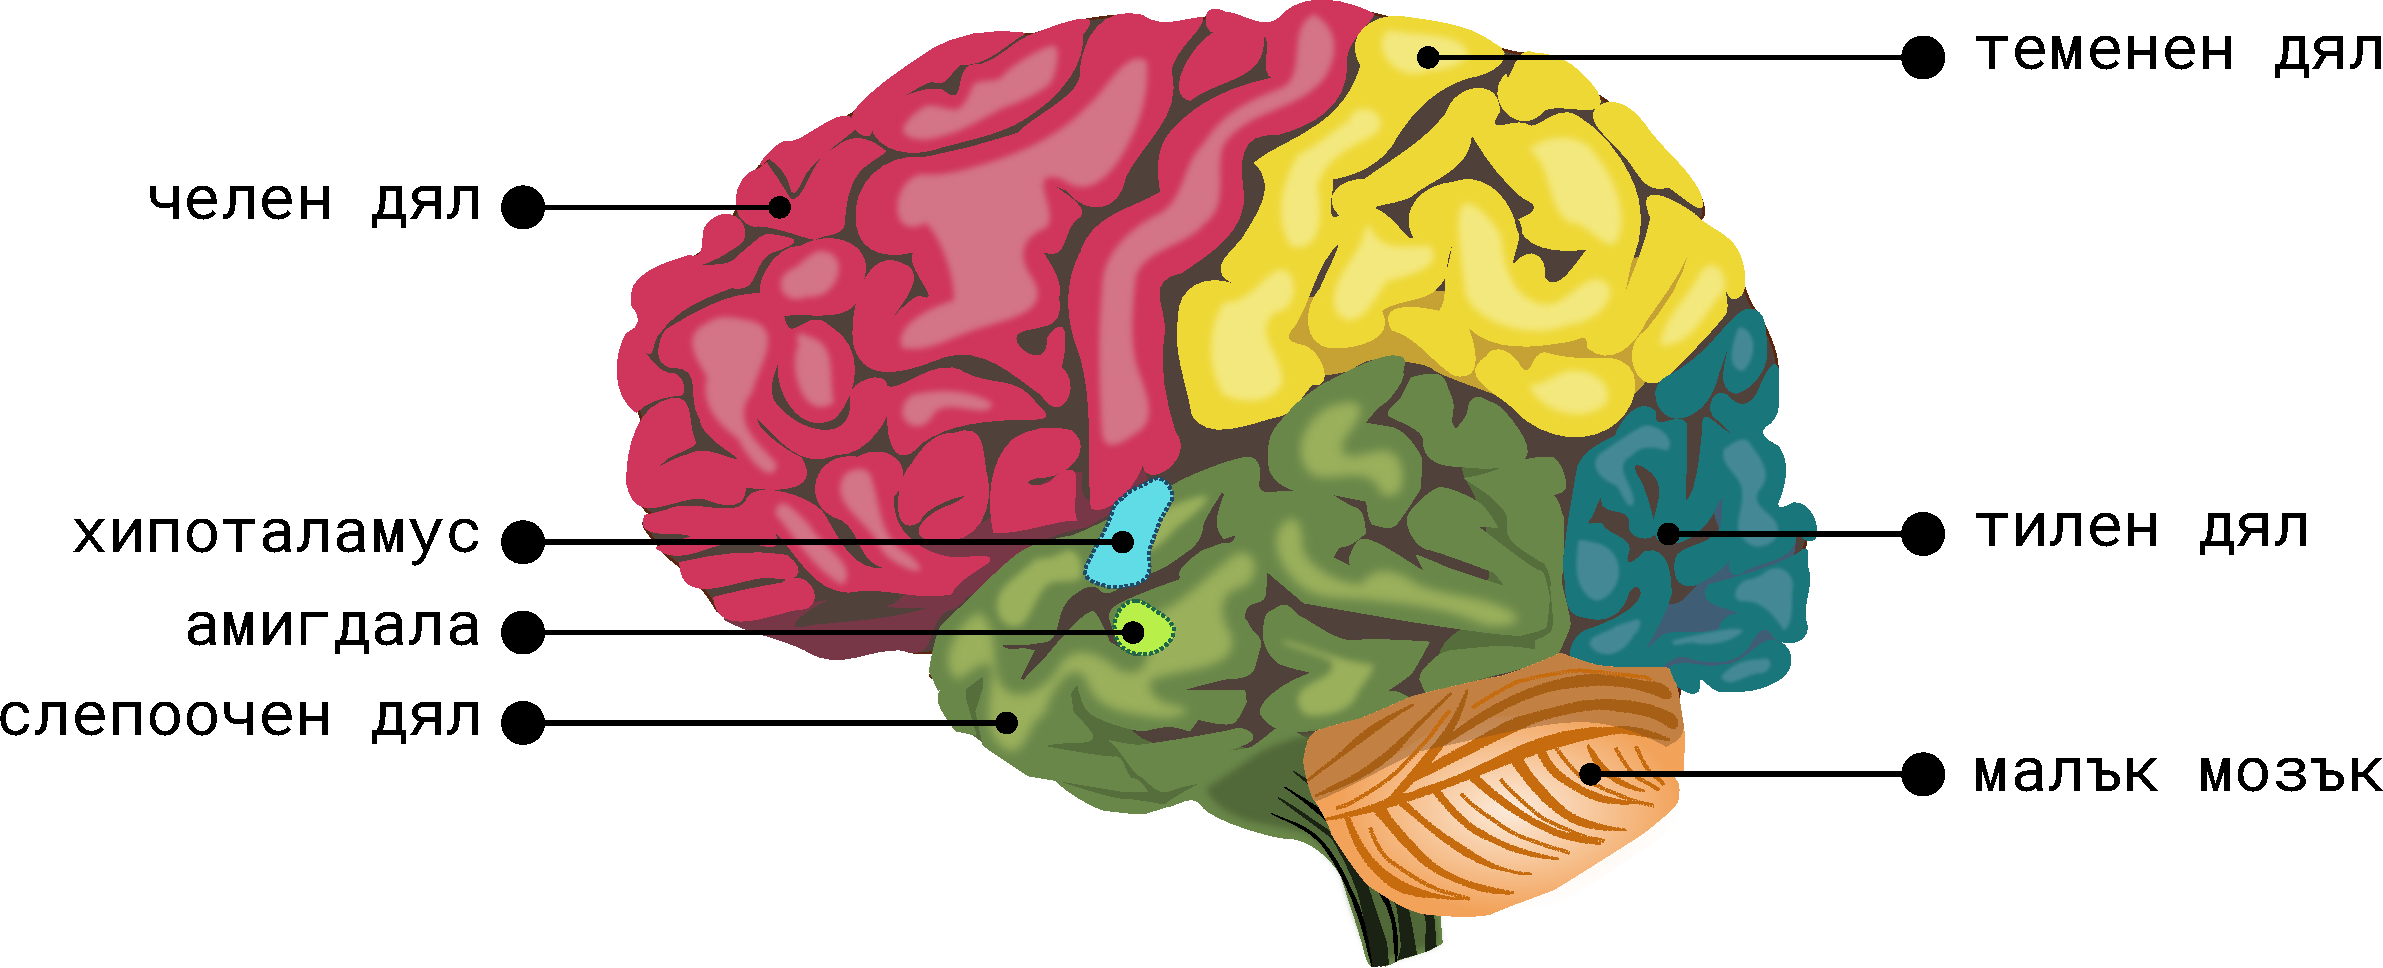
\includegraphics[width=0.75\paperwidth]{brain}}
        \only<2-4>{
            \begin{itemize}
                \item<2-4> Неврони - предават си електрически сигнали
                \item<3-4> Електроенцефалограф - измерва колебанията в напрежението на тези сигнали
                \item<4-4> Групиране на сигнала от ЕЕГ по полезни честотни ленти
            \end{itemize}
        }
        \only<5-9>{
            \begin{itemize}
                \item<5-9> $(1-4Hz)\ \delta$ вълни
                \item<6-9> $(4-8Hz)\ \theta$ вълни
                \item<7-9> $(8-12Hz)\ \alpha$ вълни
                \item<8-9> $(13-30Hz)\ \beta$ вълни
                \item<9-9> $(30-50Hz)\ \gamma$ вълни (ниски)
            \end{itemize}
        }
    \end{frame}
    
    \begin{frame}
        \only<1>{
            \center{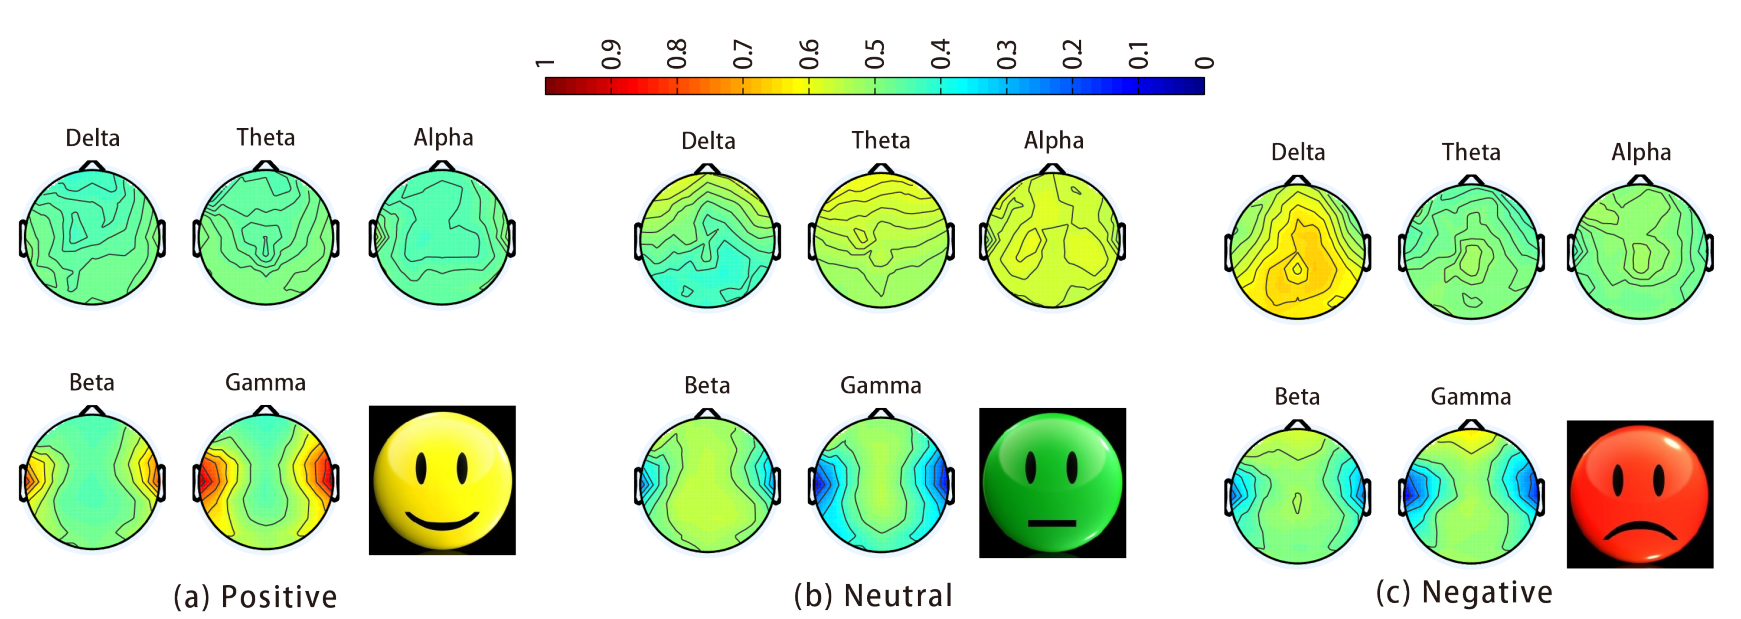
\includegraphics[width=0.8\paperwidth]{emotion_map.png}}
        }
        \only<2>{
            \center{
            \href{run:resources/georgi_video.mp4}{Видео}
            % \center{\animategraphics[loop,controls,width=0.9\linewidth]{2}{gif/all-}{0}{25}}
            }
        }
    \end{frame}
    
    \begin{frame}[t]
        \begin{columns}
            \begin{column}{0.48\textwidth}
                \center{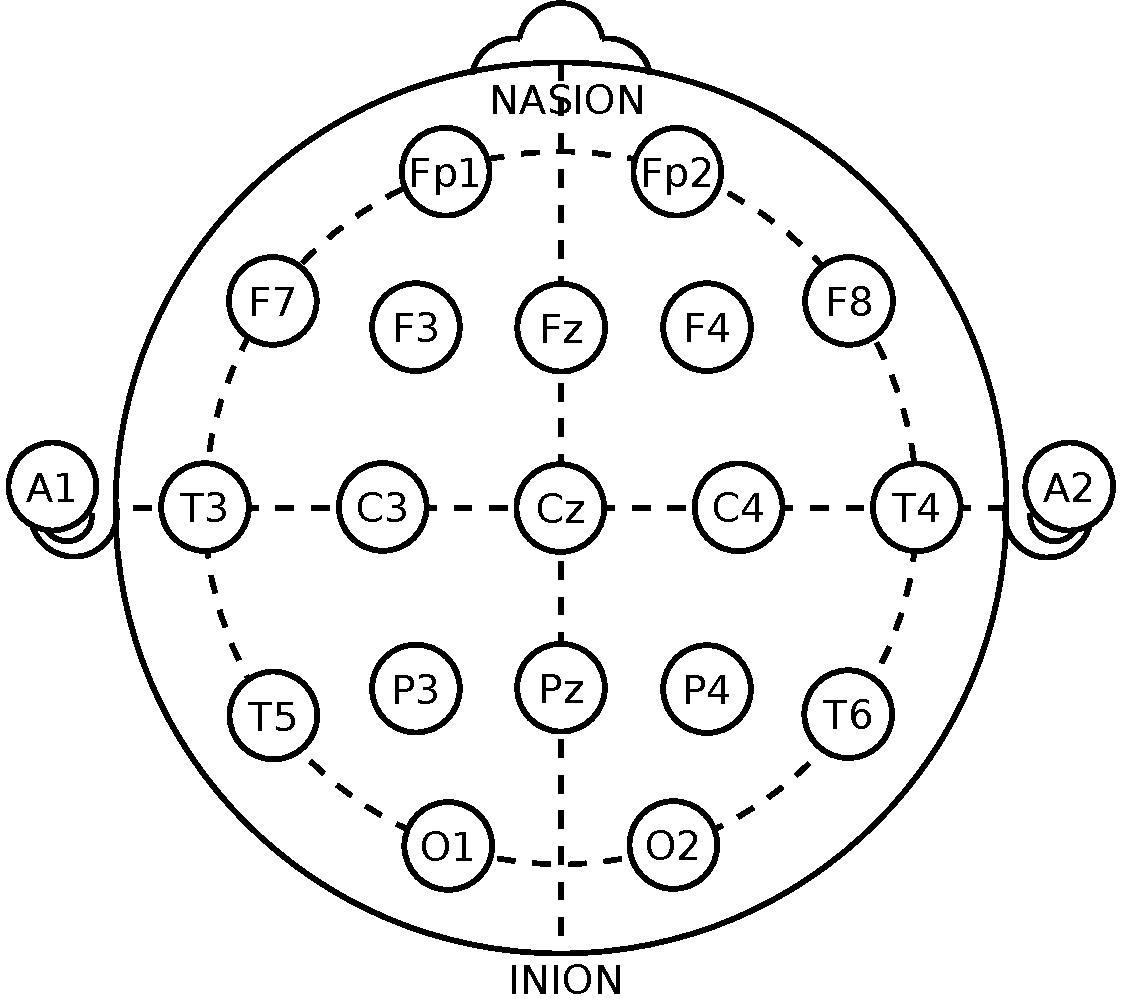
\includegraphics[width=0.8\textwidth]{10_20}}
            \end{column}
            \begin{column}{0.48\textwidth}
                \pause
                За характеристики ще ползваме енергията на  $\theta, \beta, \alpha, \gamma$ вълните
                \pause
                Енцефалографът записва $500\times19$ мерни вектора в секунда
            \end{column}
        \end{columns}
        \begin{itemize}
            \setlength\itemsep{\fill}
            \pause
            \item Прочитаме цялата информация за един електрод
            \pause
            \item Разделяме сигнала на F фрейма и разглеждаме спектъра
            \pause
            \item Сумираме енергиите в съответните 4 честотни банки, отговарящи на $\theta, \beta, \alpha, \gamma$ вълни
            \pause
            \item Получаваме F на брой $(19\times 4)$ мерни вектора
            \pause
            \item Класифицираме с Гаусови смески
        \end{itemize}
    \end{frame}

    \section{Бази данни и резултати (ЕЕГ)}
    \begin{frame}[t]{Опит едно}
        \center{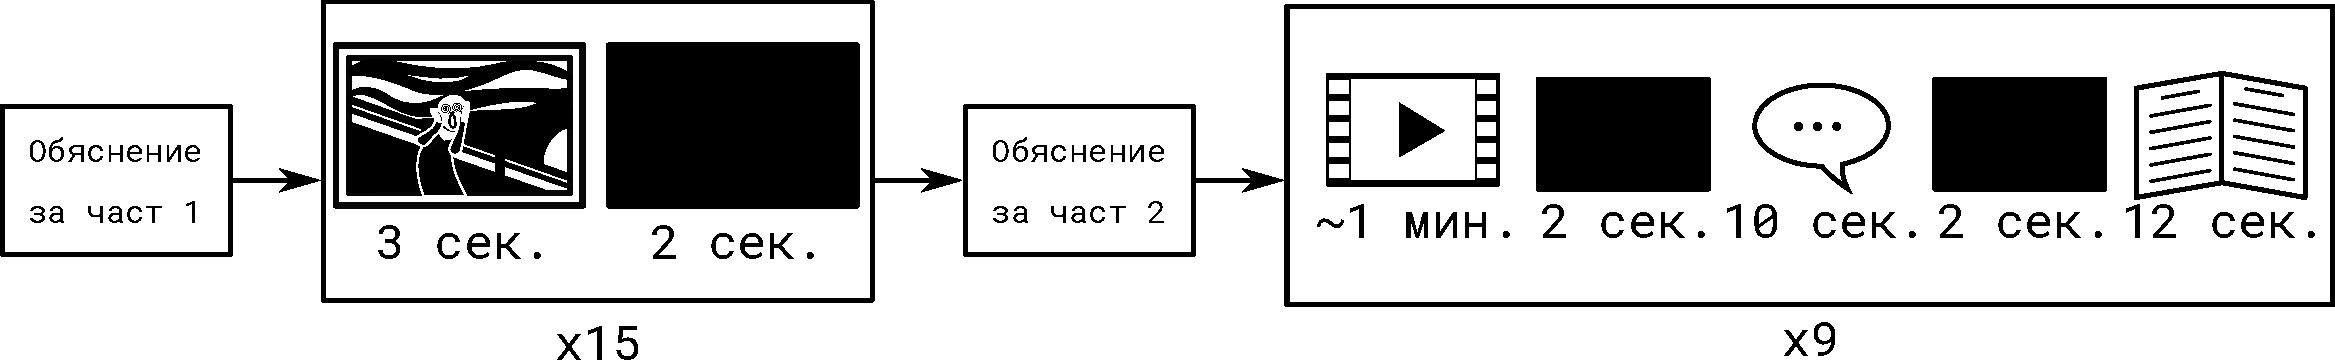
\includegraphics[width=\textwidth]{first_db}}
        \pause
        \begin{center}
        \begin{tabular}{|l|r|r|} 
            \hline
            Емоция & Брой файлове & Обща дължина\\ 
            \hline
            Гняв & 3 & 0 мин. 30 сек.\\ 
            Щастие & 3 & 0 мин. 30 сек.\\ 
            Неутрално състояние & 10 & 2 мин. 00 сек. \\ 
            Тъга & 4 & 0 мин. 40 сек. \\ 
            \hline
        \end{tabular}
        \pause
        \begin{table}[h]
            \begin{center}
            \begin{tabular}{|l|r r r r|} 
                \hline
                & Гняв & Щастие & Неутрално & Тъга \\ 
                \hline
                Гняв &  \textbf{33.33\%} & 0.00\% & 33.33\% & 33.33\% \\ 
                Щастие & 00.00\% & \textbf{100.00\%} & 0.00\% & 0.00\% \\ 
                Неутрално & 11.11\% & 0.00\% & \textbf{88.89\%} & 0.00\% \\ 
                Тъга & 0.00\% & 0.00\% & 100.00\% & \textbf{0.00\%}\\ 
                \hline
                \hline
                Общо & & & & \textbf{55.56\%}\\
                \hline
            \end{tabular}
            \caption*{Матрица на грешките от първия опит на ниво файл}
            \end{center}
        \end{table}
        \end{center}
    \end{frame}

    \begin{frame}[t]{Опит две}
            \begin{itemize}
                \pause
                \item Персонална постановка
                \pause
                \item Допълнителни стимули 
            \end{itemize}
            \pause
            \begin{center}
                \begin{tabular}{|l|r|r|} 
                    \hline
                    Емоция & Брой файлове & Обща дължина\\ 
                    \hline
                    Гняв & 18 & 6 мин. 53 сек.\\ 
                    Щастие & 0 & 0 мин. 00 сек. \\ 
                    Неутрално състояние & 31 & 8 мин. 12 сек. \\ 
                    Тъга & 45 & 15 мин. 13 сек. \\ 
                    \hline
                \end{tabular}
            \pause
            \begin{table}[h]
                \begin{center}
                    \begin{tabular}{|l|r r r r|} 
                        \hline
                        & Гняв & Щастие & Неутрално & Тъга \\ 
                        \hline
                        Гняв &  \textbf{100.00\%} & 0.00\% & 0.00\% & 0.00\% \\ 
                        Щастие & 00.00\% & \textbf{100.00\%} & 0.00\% & 0.00\% \\ 
                        Неутрално & 0.00\% & 0.00\% & \textbf{100.0\%} & 0.00\% \\ 
                        Тъга & 0.00\% & 0.00\% & 4.44\% & \textbf{95.56\%}\\ 
                        \hline
                        \hline
                        Общо & & & & \textbf{98.89\%}\\
                        \hline
                    \end{tabular}
                    \caption*{Матрица на грешките от втория опит на ниво файл}
                \end{center}
            \end{table}
            \end{center}
    \end{frame}

    \begin{frame}[c]
        \begin{center}
        \begin{table}[h]
            \begin{tabular}{|l|r r r r|} 
                \hline
                & Гняв & Щастие & Неутрално & Тъга \\ 
                \hline
                Гняв &  \textbf{80.33\%} & 5.00\% & 15.33\% & 0.00\% \\ 
                Щастие & 25.00\% & \textbf{75.00\%} & 0.00\% & 0.00\% \\ 
                Неутрално & 0.00\% & 2.50\% & \textbf{97.50\%} & 0.00\% \\ 
                Тъга & 0.00\% & 2.08\% & 10.42\% & \textbf{87.50\%}\\ 
                \hline
                \hline
                Общо & & & & \textbf{85.00\%}\\
                \hline
            \end{tabular}
            \caption*{Матрица на грешките при комбиниране на данните от първия и втория опит на ниво файл}
        \end{table}
        \end{center}
    \end{frame}

    \section{Реч и ЕЕГ}
    \begin{frame}[t]
        \begin{itemize}
            \item Идея едно
            \pause - конкатенираме характеристичните вектори от двата сигнала и тренираме нов класификатор
        \end{itemize}
        \pause
        \begin{table}[h]
            \begin{center}
                \resizebox{0.7\textwidth}{!}{\begin{tabular}{|l|r r r|}
                    \hline
                    Емоция    & Само реч         & Само ЕЕГ         & Конкатенация     \\
                    \hline
                    Гняв      & 85.00\%          & 80.00\%          & 86.50\%          \\
                    Щастие    & 75.00\%          & 75.00\%          & 57.50\%          \\
                    Неутрално & 7.50\%           & 97.50\%          & 91.75\%          \\
                    Тъга      & 85.42\%          & 87.50\%          & 81.04\%          \\
                    \hline
                    \hline
                    Общо      & \textbf{63.23\%} & \textbf{85.00\%} & \textbf{79.20\%} \\
                    \hline
                \end{tabular}}
                \caption*{Ниво файл}
            \end{center}
        \end{table}
    \end{frame}

    \begin{frame}[t]
        \begin{itemize}
            \setlength\itemsep{\fill}
            \item Идея две
            \pause - принцип за максимизиране на ентропията
            
            \pause Като правим заключения на базата на частична информация, трябва да използваме това разпределение, което има максимална ентропия, спрямо известните величини.
            \pause 
            \item Може да се покаже, че това разпределение максимизира и логаритъм от условното правдоподобие
            \pause $\log\B{\widehat{L}_{\mathcal{D}}(Y|X)} = \sum\limits_{(x, y) \in X\times Y} \#(x, y) p(y|x)$
            \pause
            \item и че има вида има вида:
            \pause
            \[\hat{p}(y|x) = \cfrac{exp\B{\lambda_1 h_1(x, y) + \lambda_2 h_2(x, y)}}{\sum\limits_{y' \in Y} exp\B{\lambda_1 h_1(x, y') + \lambda_2 h_2(x, y')} }\]
            \pause
            \item Намираме $\lambda_1, \lambda_2$ с градиентен метод от първи ред
            \pause
            \item Получаваме следния класификатор:
            \pause \[H(x) = argmax_{y\in Y} \B{\lambda_1 h_1(x, y) + \lambda_2 h_2(x, y)}\]
        \end{itemize}
    \end{frame}

    \begin{frame}[t]
        \begin{table}[h]
        \begin{center}
            \begin{tabular}{|l|r r r|}
                \hline
                Емоция    & Само реч         & Само ЕЕГ         & Комбинация     \\
                \hline
                Гняв      & 85.00\%          & 80.00\%          & 80.00\%          \\
                Щастие    & 75.00\%          & 75.00\%          & 75.00\%          \\
                Неутрално & 7.50\%           & 97.50\%          & 97.50\%          \\
                Тъга      & 85.42\%          & 87.50\%          & 87.50\%          \\
                \hline
                \hline
                Общо      & \textbf{63.23\%} & \textbf{85.00\%} & \textbf{85.00\%} \\
                \hline
            \end{tabular}
            \caption*{Ниво файл}
        \end{center}
        \end{table}
        \pause
        \begin{table}[h]
            \begin{center}
                \begin{tabular}{|l|r r r|}
                    \hline
                    Емоция    & Само реч         & Само ЕЕГ         & Комбинация     \\
                    \hline
                    Гняв      & 41.53\%          & 53.05\%          & 53.30\%          \\
                    Щастие    & 37.35\%          & 44.44\%          & 44.09\%          \\
                    Неутрално & 32.91\%           & 66.72\%          & 66.46\%          \\
                    Тъга      & 39.66\%          & 70.38\%          & 71.07\%          \\
                    \hline
                    \hline
                    Общо      & \textbf{37.86\%} & \textbf{58.65\%} & \textbf{58.73\%} \\
                    \hline
                \end{tabular}
                \caption*{Ниво вектор}
            \end{center}
        \end{table}
    \end{frame}

    \section{Заключение}
    \begin{frame}[t]
        \begin{tikzpicture}[remember picture,overlay]
            \node at (current page.center) {
\includegraphics[width=\paperwidth]{3.png}};
        \end{tikzpicture}
        \begin{center}
            \textbf{Заключението, което можем да направим, е, че с тази постановка съчетаването на двата сигнала не довежда до подобрение.}
        \end{center}
        \vspace{5cm}
        \begin{center}
            {\footnotesize Сбогом и благодаря за рибата!}
        \end{center}
    \end{frame}
\end{document}